\section{Evaluation}\label{sec:evaluation}

% We present the discovered sources of unsafety and their evaluation on the examined tools. 
% We present our answers to the two major research questions solved in this paper. We start with our
% discovered sources of unsafety in the examined tools, using the \ac{poc} repository approach.
% Afterwards, we display the occurrence of some of the discovered sources of unsafety in the wild by
% presenting the results of our broad open source project scan. Combining the gained knowledge, we
% present common patterns and examples that were found to be significant sources of unsafety.

\subsection{RQ1 \& RQ2: Sources of Unsafety for the Examined \ac{rts}-Tools}
Using the \ac{poc} repository approach described in Section~\ref{ssec:pocs}, we were able to
test all proposed sources of unsafety with the examined \ac{rts}-tools. The results are shown in
Table~\ref{table:poc_results}. We evaluated the Spring and Guice \ac{di} frameworks separately,
because their different implementations lead to different test results.
Hypothesis~\ref{hyp:dep_inj:external} was not tested separately, because the \ac{poc} repository for
hypothesis~\ref{hyp:external_files} and its tests already cover external file changes as sources of
unsafety. This superset of unsafety already includes unsafety from changed external configuration
files for dependency injection.

While executing the testing procedure described in Section~\ref{ssec:pocs}, we came across
more problems with some of the examined tools that prevented us from collecting all test results.
\footnote{The version of \emph{Ekstazi} that is used by \emph{GIBstazi} does not support method
calls to \texttt{Class.getTypeName(...)}. \emph{GIBstazi} therefore cannot run tests using the
JUnit test runner \texttt{SpringRunner} required for testing Spring framework
functionality.\label{foot:**}}
\footnote{\emph{OpenClover} cannot detect tests run with the \texttt{SpringRunner}.\label{foot:***}}
\footnote{The latest version of \emph{Ekstazi} (version 5.3.0) is incompatible with the latest
version of Guice (version 5.0.1). This problem with \emph{Ekstazi} is evaluated separately in
Section~\ref{ssec:runtime_instrumentation}. All tests with \emph{Ekstazi} and the Guice framework
therefore use Guice version 4.2.3, which is currently the latest version that is supported by
\emph{Ekstazi}.\label{foot:****}}
These problems
have the potential of leading to sources of unsafety themselves and should therefore be the subject
of further studies.

\begin{savenotes}
    \begin{table}[h]
        \caption{Test results of \ac{poc} repository tests, uncovering sources of unsafety in examined
            \ac{rts}-tools.}\label{table:poc_results}
        \centering
        \begin{tabular}{l | c | c | c | c | c}
            \hline
            Hypothesis                                                  & \emph{Ekstazi}              & \emph{GIBstazi}             & \emph{OpenClover}         & \emph{STARTS} & \emph{HyRTS} \\
            \hline
            \ref{hyp:dyn_dis}: Dynamic Dispatch                         & $\times$                    & $\times$                    & $\checkmark$              & $\times$      & $\times$     \\
            \ref{hyp:external_files}: External Files                  & $\checkmark$                & $\times$                    & $\checkmark$              & $\checkmark$  & $\checkmark$ \\
            \ref{hyp:config_files}: Configuration Files               & $\checkmark$                & $\times$                    & $\checkmark$              & $\times$      & $\checkmark$ \\
            \ref{hyp:reflections}: Reflections                 & $\times$                    & $\times$                    & $\times$                  & $\checkmark$  & $\checkmark$ \\
            \ref{hyp:static_init}: Static Initializers            & $\checkmark$                & $\checkmark$                & $\checkmark$              & $\checkmark$  & $\checkmark$ \\
            \ref{hyp:dep_inj:source}: Dependency Injection (Spring)      & $\times$                    & \danger\footref{foot:**}    & \danger\footref{foot:***} & $\checkmark$  & $\times$     \\
            \ref{hyp:dep_inj:source}: Dependency Injection (Guice)       & $\times$\footref{foot:****} & $\times$\footref{foot:****} & $\times$                  & $\checkmark$  & $\times$     \\
            \ref{hyp:dep_inj:collections}: Collection Injection (Spring) & $\checkmark$                & \danger\footref{foot:**}    & \danger\footref{foot:***} & $\checkmark$  & $\checkmark$ \\
            \ref{hyp:dep_inj:collections}: Collection Injection (Guice)  & $\times$\footref{foot:****} & $\times$\footref{foot:****} & $\times$                  & $\times$      & $\checkmark$ \\
            \ref{hyp:dep_inj:scan}: Spring AutoConfiguration            & $\checkmark$                & \danger\footref{foot:**}    & \danger\footref{foot:***} & $\checkmark$  & $\checkmark$ \\
            \ref{hyp:dep_inj:scan}: Spring ComponentScan                & $\checkmark$                & $\checkmark$                & $\checkmark$              & $\checkmark$  & $\checkmark$ \\
            \ref{hyp:instrumentation}: Runtime Instrumentation      & $\checkmark$                & $\checkmark$                & $\checkmark$              & $\times$      & $\times$     \\
            \hline
        \end{tabular}
        \caption*{Legend:\\$\times$: The hypothesis does not hold, the tool is not susceptible to this
                source of unsafety;\\$\checkmark$: The hypothesis does hold, this tool is unsafe;\\
            \danger: No usable result was produced.}
    \end{table}
\end{savenotes}

Most of the presented sources of unsafety are undocumented for the examined tools. The \emph{STARTS} tool
documented problems with reflections~\cite{starts_paper} as their only known source of unsafety in
comparison to the \emph{Ekstazi} tool. That is the reason why especially
unsafety occurring with the \emph{Ekstazi} \ac{rts}-tool poses a great risk. Studies about newly
developed \ac{rts}-tools
often use it for comparisons of their selected test sets to determine their tool's safety and
precision.\cite{prestarts,starts_paper,hyrts_paper,gibstazi_paper}.

In contrast to the paper published about the \emph{Ekstazi} tool~\cite{ekstazimain}, our research shows that even the latest
version of the \ac{rts}-tool is not able to track changes in external files and configuration files.
The tool's published source code contains a disabled \texttt{FileRecorder} class that could be used
to replace Java's default \texttt{SecurityManager} class. However, when we manually activated and
tested\footnote{These specific tests
were executed with the Java SE JDK Version 8, running on an Ubuntu 21.10 operating
system with the 5.13.0 Linux Kernel.} this supposedly
linux-specific feature, Ekstazi was still not able to detect file access via \texttt{java.io} or
\texttt{java.nio} functions. This file recording feature is disabled by default and not shipped with
the \ac{rts}-tool.

\emph{GIBstazi}, being a wrapper that mainly combines the GIB tool with \ac{rts} performed by \emph{Ekstazi},
inherits most problems that occur with \emph{Ekstazi}. External files however are detected, because
\emph{GIBstazi} executes all tests from a module if an external file was modified~\cite{gibstazi_paper}.
Besides that, the included, outdated version of \emph{Ekstazi} leads to additional problems with modern
test runners.

\subsection{RQ3 \& RQ4: Sources of Unsafety in the Wild}\label{ssec:eval:3_4}

With the commit scanners defined in Section~\ref{sssec:repo_scanning} we were able to detect
several previously described sources of unsafety in open source projects in the wild. Out of the $100$
examined projects, $88$ included a source of unsafety in their 100 latest commits. $8$ of these
repositories even contained each of the searched sources of unsafety at least once. An overview of
the number of sources of unsafety discovered in each project is shown in Figure~\ref{fig:box_plot}.

\begin{figure}[h]
    \caption{Sources of unsafety per repository, discovered in repositories and commits collected in
        Section~\ref{sec:foss_search}. (Removed outliers above 75 sources of unsafety. The
        full diagram is shown in Figure~\ref{appx:fig:box_plot})}\label{fig:box_plot}
    \centering
    \vspace{2em}
    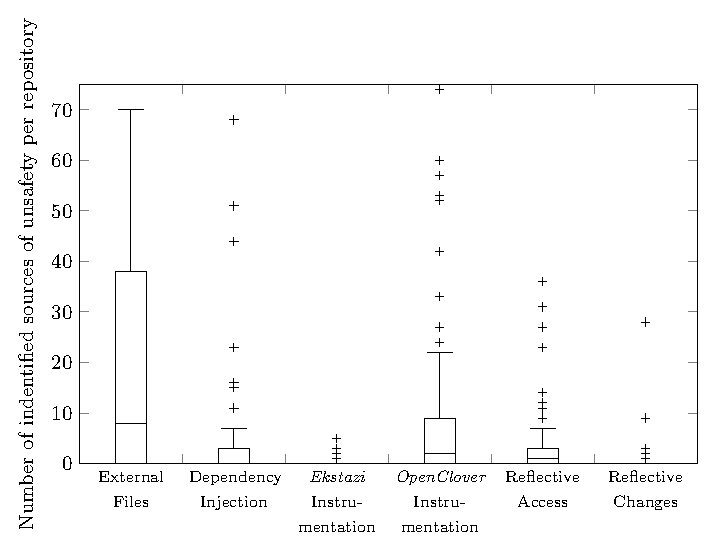
\includegraphics[scale=0.9]{./figures/pdf/box_plot.pdf}
\end{figure}

Figure~\ref{fig:probs_commits} visualizes the composition of sources of unsafety on a commit-level.
Unsafety produced by runtime instrumentation is not included in the graphic. It is
not caused by changes introduced in a commit, but by the underlying code base that contains the
problematic method calls. We also only recorded all appearances of the \texttt{Class.forName(...)}
method call for every commit without explicitly documenting the changes between commits. We used
this data to infer changes between commits, which also means that we do not have change data for
the first scanned commit of every repository.

\begin{figure}[h]
    \caption{Absolute number of commits that contain the associated source of unsafety (over all projects).}\label{fig:probs_commits}
    \centering
    \vspace{2em}
    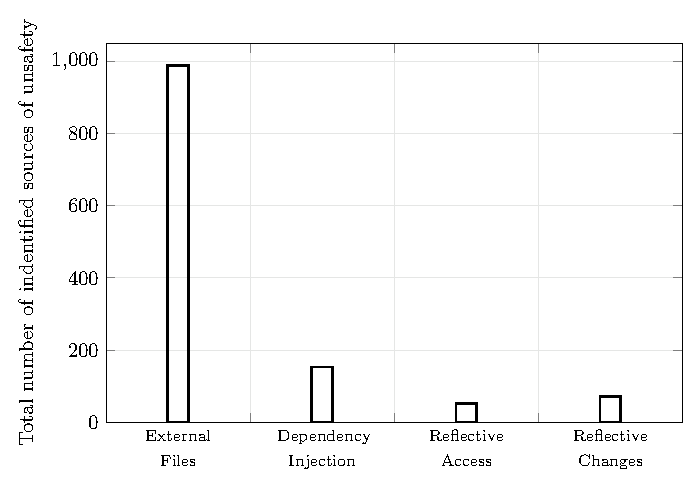
\includegraphics[scale=0.7]{./figures/pdf/commit_bar.pdf}
\end{figure}

\subsubsection{External Files}
With this scanner, we identified a total of $989$ commits that change an average of
$11.85$ external files in the searched paths. The commits change, on average, $1993.59$ lines of
text in the external files. This number only includes changes on external files whose content is
versioned via git. Even though most of these file changes may not change the program's behavior,
they all are sources of unsafety, because their changes are not detected by most of the examined
\ac{rts} tools.

\subsubsection{\acf{di}}
Of the $100$ examined projects, $53$ depend on libraries from the Spring framework, $17$ on Guice
libraries, $5$ on the CDI \ac{di} implementation and $3$ on the Dagger \ac{di} framework. This shows
that \ac{di} is an important factor in evaluating the unsafety of \ac{rts}-tools.

For in-depth scans, we concentrated on Spring and Guice \ac{di} features. We recorded $484$ changes on
Spring-related and $297$ changes on Guice-related keywords (listed in
Table~\ref{table:dep_inj_keywords}). None of the examined repositories uses Guice in combination with the
Netflix Governator library that allows for automatic classpath scanning.

\subsubsection{Runtime Instrumentation}
This scanner identified $63$ programs whose behavior changes due to the
profiling and coverage approaches used by \emph{Ekstazi} and \emph{OpenClover}. $11$ repositories
contain code that cannot be executed with \emph{Ekstazi}'s runtime instrumentation enabled. 
\emph{OpenClover} changes the behavior of
code in $49$ repositories. $3$ projects contain code that is affected by both tools. 
With, on average, $14.80$ incompatible files per
affected repository, this source of unsafety normally renders the corresponding tool unusable for
the project. Though, if the repository still uses the tool, the resulting differences in test
results can cause correctly failing tests to pass and vice versa.

\subsubsection{Reflections}
We mainly scanned for appearances of the \texttt{Class.forName(...)} method call
that is the main reason for most reflection-related unsafety. Other methods of reference to meta
class instances require a static method call on the class that creates a solid dependency. $56$
of the projects use this method at least once, but in general between $1$ and $36$ times. We counted
$333$ occurrences across all repositories. In addition to this search, we also tried to follow the
loaded class paths and detect changes on these classes that loaded via reflections. The problems
with this approach are described in Section~\ref{scanner:reflections}. We were able to
detect a total of $72$ changes on classes that are loaded via reflections in $8$ projects. These
changes are undetected by \emph{STARTS} and \emph{HyRTS}. Their
static initialization is also undetected by all examined tools, making them a major, so far
undocumented source of unsafety.

% Things to note:
% - Commit hashes are excepted to be unique among all projects
% - Runtime instrumentation was only recorded project wide and is therefore not respected for commit-level analysis
% - Reflection access was also only recorded on a project level but was calculated back to changes -> missing changes from first commit!
% - Of the 10000 commits, 1151 commits introduced unsafe behavior (runtime instrumentation ignored) -> 11.51\%
% How many projects are free of detected unsafety? Which projects contain all sources of unsafety?
